\documentclass{beamer}
\usepackage{graphicx}
\usepackage{tikz}
\usetikzlibrary{shapes,arrows}
\usepackage{tikz}
\usetheme{tg}

%\usecolortheme{seahorse}
  \setbeamertemplate{footline}[page number]
\usepackage{multirow}
\setbeamertemplate{navigation symbols}{}
\setbeamertemplate{frametitle}[default][center]
\setbeamerfont{frametitle}{shape=\scshape}
\usepackage{color}

\usepackage{csquotes}

\usepackage{xcolor}

\usepackage[flushleft]{threeparttable}

{\title{\textsc{Econ 352 - International Trade in Goods and Assets} \\ \tiny (See Williamson Ch. 16)}
\author{Trevor S. Gallen}
\date{}
\begin{document}
\renewcommand*{\inserttotalframenumber}{\pageref{lastframe}}


\setbeamertemplate{caption}{\raggedright\insertcaption\par}

\begin{frame}
\titlepage
\end{frame}

\begin{frame}
\frametitle[alignment=center]{Introduction}
\begin{itemize}
\item We have a model with nominal prices, discussed New Keynesian model, etc.
\bigskip
\item But so far our model has just been of one country, no trade
\bigskip
\item Now we'll model  a ``small open economy," an economy that trades but isn't big enough to affect prices in other countries
\bigskip
\item We'll discuss what drives ``current account surpluses," savings above investment
\end{itemize}
\end{frame}

\begin{frame}
\frametitle[alignment=center]{Current Account}
\begin{itemize}
\item Rep. consumer has usual present-value budget constraint:
$$C+\frac{C'}{1+r}=Y-T+\frac{Y'-T'}{1+r}$$
\item Where private savings is thus:
$$S^p=Y-T-C$$
\item Government's present-value budget constraint is:
$$G+\frac{G'}{1+r}=T+\frac{T'}{1+r}$$
\item And government savings is:
$$S^G=T-G$$
\item If we shut down investment, all savings is the current account:
$$CA=S-I=(S^P+S^G)-0=(Y-T-C)+(T-G)=Y-C-G$$
\item If we had investment (which we'll ignore) it would have been:
$$CA=Y-C-G-I$$
\end{itemize}
\end{frame}


\begin{frame}
\frametitle[alignment=center]{Combine Consumer \& Govt}
\begin{itemize}
\item Adding up the consume and govt budget constraints to get the national present-value budget constraint:
$$C+\frac{C'}{1+r}+G+\frac{G'}{1+r}=Y+\frac{Y'}{1+r}$$
\item Just like we would have had $Y=C+G+I$, now we have:
$$Y=C+G+CA$$
$$Y'+(1+r)CA=C'+G'$$
\item So the CA acts like national savings.
\smallskip
\item We'll generally ignore C vs G, combine into $C+G$
\smallskip
\item Graphing the national budget constraint, we get:
\end{itemize}
\end{frame}


\begin{frame}
\frametitle[alignment=center]{National PV Budget Constraint}
\begin{figure}
\centering
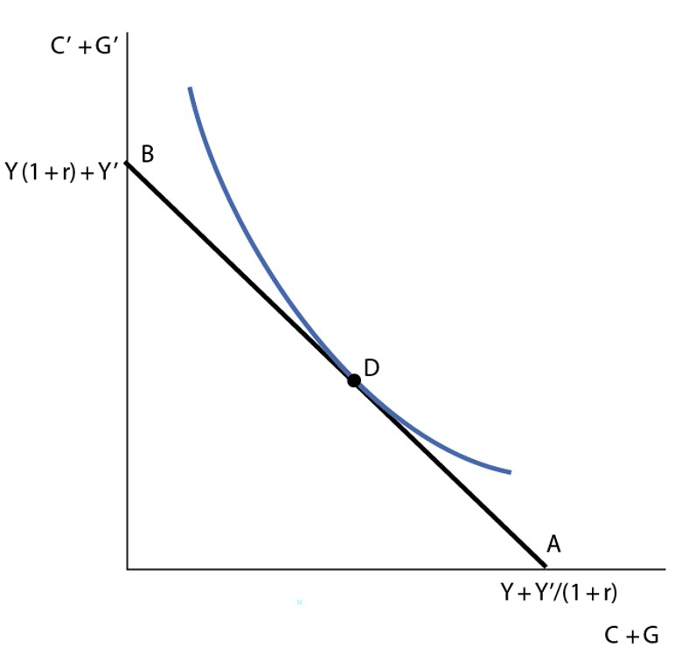
\includegraphics[scale=0.75]{Figures/W_Fig_16pt1.png}
\end{figure}
\end{frame}

\begin{frame}
\frametitle[alignment=center]{National Savings-I}
\begin{itemize}
\item Current account is national savings (when we exclude investment)
\bigskip
\item Note that this problem looks just like Chapter 9's household intertemporal problem
\bigskip
\item Current account is just like savings, so we can analyze it in same way!
\end{itemize}
\end{frame}

\begin{frame}
\frametitle[alignment=center]{National Savings-II}
\begin{itemize}
\item Five predictions about national savings excluding investment (current account)
\bigskip
\begin{enumerate}
\item Current account surplus rises with an increase in current income (smoothing!)
\smallskip
\item Current account surplus falls with an increase in future income (smoothing!)
\smallskip
\item Tax changes, holding constant govt spending, should not effect current account surplus (no change in BC, no change in allocation!)
\smallskip
\item If current account surplus is less than zero (dissaving), then an increase in the interest rate increases CA (inc \& sub same direction)
\smallskip
\item If a current account surplus is greater than zero (savings) then an increase in the interest rate has an ambiguous effect on current account (conflicting inc and sub effects)
\end{enumerate}
\end{itemize}
\end{frame}




\begin{frame}
\frametitle[alignment=center]{Credit Market Imperfections and Default}
\begin{itemize}
\item So far, debt (current account deficits) aren't such a big deal
\bigskip
\item But national default is a big deal!
\bigskip
\item Think about limited commitment, in which a country can walk away from its debts
\bigskip
\item Letting $B$ be debt, the budget constraint is:
$$C+G=Y+\frac{B'}{1+r}-B$$
\item And the future budget constraint:
$$C'+G'=Y'-B'$$
\item Where $B'$ is the newly-issued debt in the first period (income then, debt next period)
\end{itemize}
\end{frame}


\begin{frame}
\frametitle[alignment=center]{Credit Market Imperfections and Default-II}
\begin{itemize}
\item Combining the budget constraints, we get:
$$C+\frac{C'}{1+r}+G+\frac{G'}{1+r}=Y+\frac{Y'}{1+r}-B$$
\item And the current account in the first period is the change in indebtedness (net new resources from abroad):
$$CA=B-\frac{B'}{1+r}$$
\bigskip
\item We live in a world of limited commitment, like in Chapter 10:  countries can walk away from debt.
\bigskip
\item Can't post collateral, but can be punished (pursued in debt markets, for instance), call this penalty $v$, like collateral:
$$-B'\leq \nu$$
\end{itemize}
\end{frame}

\begin{frame}
\frametitle[alignment=center]{Credit Market Imperfections and Default-III}
\begin{itemize}
\item We have the non-default constraint on debt:
$$-B'\leq \nu$$
\item Which, plugged into the first period budget constraint, gives:
$$C+G\leq Y-B+\frac{\nu}{1+r}$$
\item Country has a choice of default:  if default, don't pay $B$, but get locked out of debt markets ($B'=0$) and suffer penalty ($\nu$)
\bigskip
\item Graph out two problems: intetermporal b.c's with and without default
\end{itemize}
\end{frame}

\begin{frame}
\frametitle[alignment=center]{Default Optimal}
\begin{itemize}
\item Two choices, default or don't
\bigskip
\item Assume country would have borrowed maximum amount if it doesn't default, so $B'=v$
\bigskip
\item In that case, $(C+G)_1=Y-B+\frac{v}{1+r}$, and $(C+G)_2=Y'-v$ (pay $v$ because $B'=v$)
\bigskip
\item Or we could default:  $(C+G)_1=Y$ (pay off no debt), and $(C+G)_2=Y'-v$ (now pay $v$ b/c default)
\bigskip
\item Obviously default is optimal here
\end{itemize}
\end{frame}



\begin{frame}
\frametitle[alignment=center]{Default}
\begin{figure}
\centering
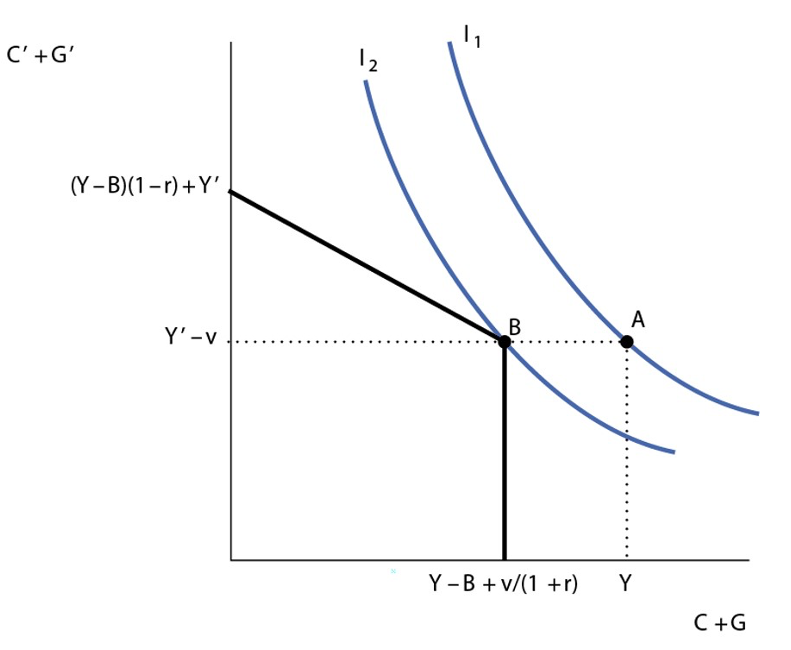
\includegraphics[scale=0.7]{Figures/W_Fig_16pt3.png}
\end{figure}
\end{frame}


\begin{frame}
\frametitle[alignment=center]{Default Not Optimal}
\begin{itemize}
\item Two choices, default or don't
\bigskip
\item Say $v$ is very high, so can borrow a lot, and $Y$ is low, so want to borrow
\bigskip
\item In that case, default gets: $(C+G)_1=Y$, $(C+G)_2=Y'-v$
\bigskip
\item And no default gets: $(C+G)_1=(Y-B+v/(1+r))$ and $(C+G)_2=Y'-v$
\bigskip
\item Key is if $v$ is big, shifts out budget constraint and makes us happier
\end{itemize}
\end{frame}

\begin{frame}
\frametitle[alignment=center]{Default not optimal}
\begin{figure}
\centering
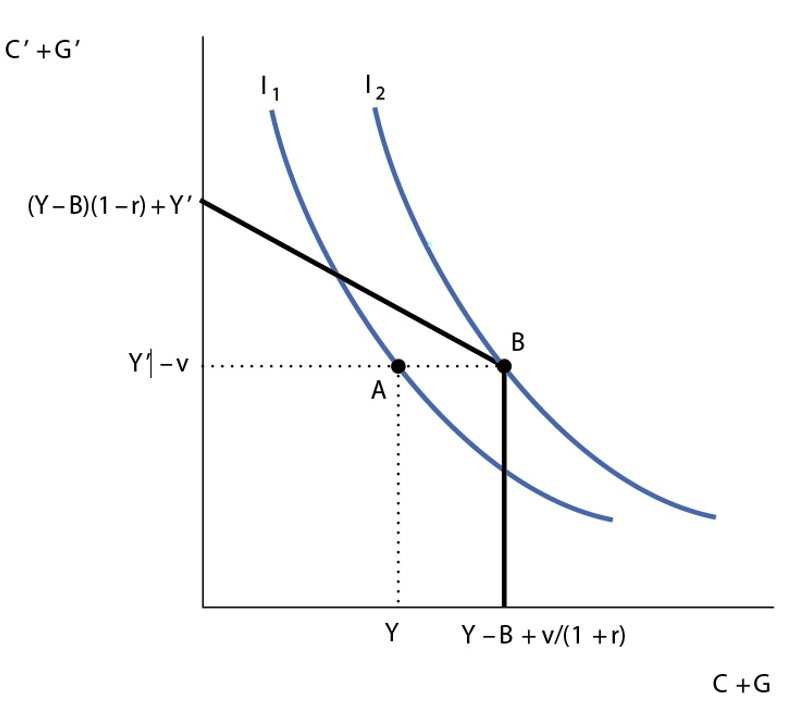
\includegraphics[scale=0.7]{Figures/W_Fig_16pt4.png}
\end{figure}
\end{frame}




\begin{frame}
\frametitle[alignment=center]{Making Sense of Default vs Not}
\begin{itemize}
\item If limited commitment holds, we have the budget constraints:
$$C+G=Y-B+\frac{\nu}{1+r}$$
$$C'+G'=Y-\nu$$
\item Total consumption in future is always same no matter what (either pay back $\nu$ or lose $\nu$ b/c didn't pay back)
\bigskip
\item So, we default only based on what default does to today's consumption (does nothing to tomorrow).  We compare consumption under no default against consumption under default:
$$Y-B+\frac{\nu}{1+r}<Y$$
\item Which says we default if and only if:
$$B>\frac{\nu}{1+r}$$
\item When debt is higher, should default, when pain of default higher, don't default
\end{itemize}
\end{frame}




\begin{frame}
\frametitle[alignment=center]{Is Current Account Deficit Bad?}
\begin{itemize}
\item Borrowing seems bad
\bigskip
\item But it has its uses (particularly when investing, but also when smoothing)
\bigskip
\item Let's see if the U.S. uses its current account deficit to smooth consumption (when GDP low, is CA also low?)
\end{itemize}
\end{frame}


\begin{frame}
\frametitle[alignment=center]{Current account negatively correlated with GDP??}
\begin{figure}
\centering
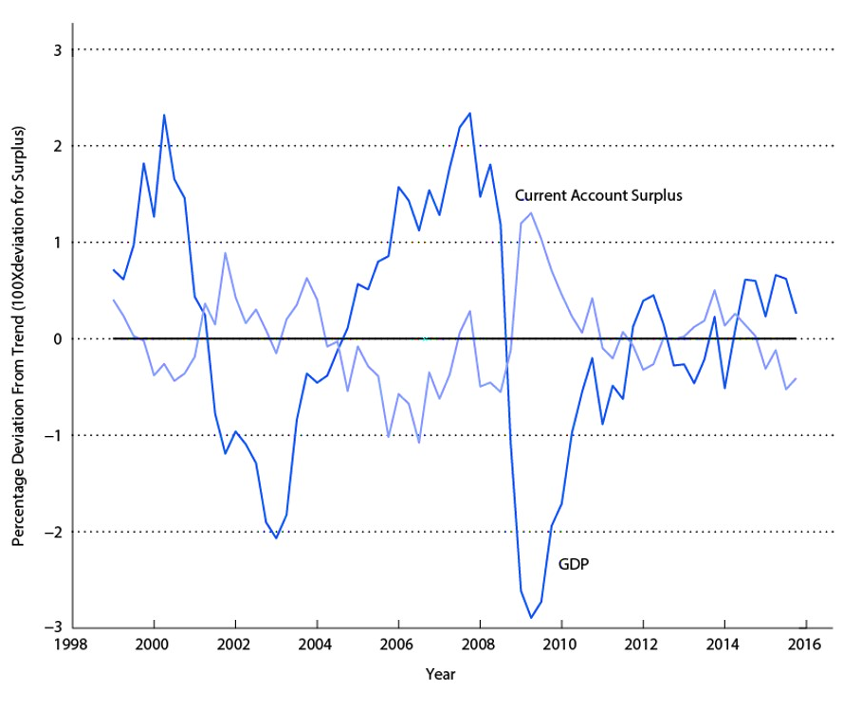
\includegraphics[scale=0.7]{Figures/W_Fig_16pt2.png}
\end{figure}
\end{frame}



\begin{frame}
\frametitle[alignment=center]{Is Current Account Deficit Bad-II}
\begin{itemize}
\item Should think about total savings, which includes investment!
\end{itemize}
\end{frame}

\begin{frame}
\frametitle[alignment=center]{Current Account vs Investment}
\begin{figure}
\centering
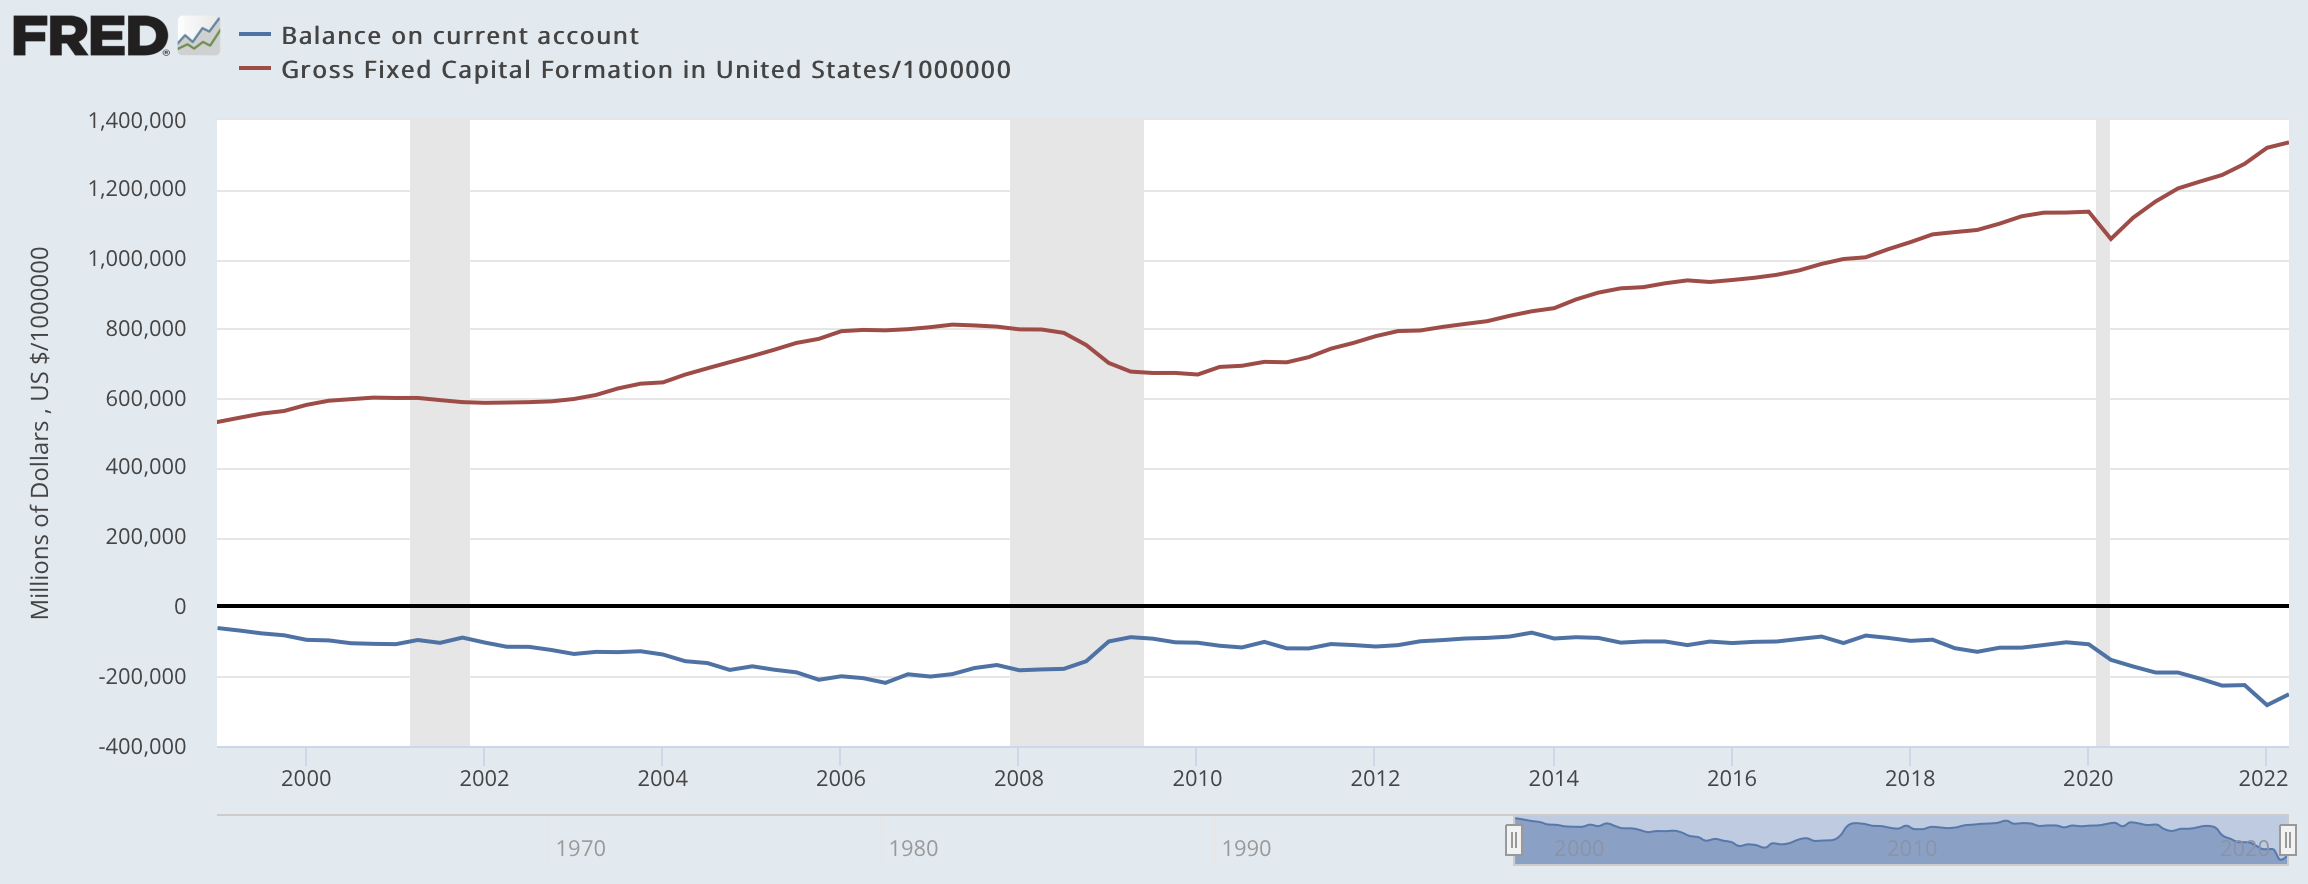
\includegraphics[scale=0.27]{Figures/CurrentAccount.png}
\end{figure}
\end{frame}

\begin{frame}
\frametitle[alignment=center]{Greece and Sovereign Default}
\begin{itemize}
\item In 2001, Greece abandoned the Drachma and began using the Euro
\bigskip
\item Before that, its debt traded at a higher interest rate (lower price for lenders) than Germany's
\bigskip
\item These differences are likely due to a fear of default (explicit or via inflation)
\bigskip
\item But 2008 and after, Greece was in a bad situation, and the possibility it would default spiked: interest rates followed that spike 
\bigskip
\item Let's take a look!
\end{itemize}
\end{frame}


\begin{frame}
\frametitle[alignment=center]{Greece and Sovereign Default}
\begin{figure}
\centering
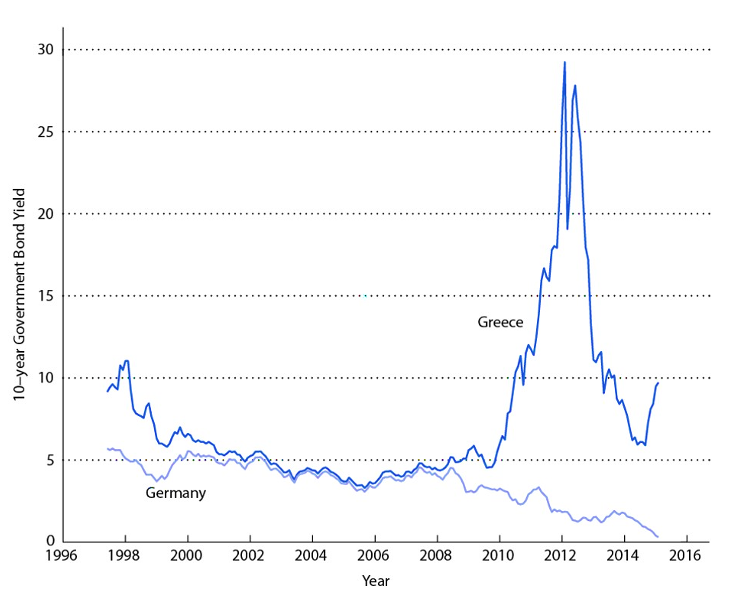
\includegraphics[scale=0.7]{Figures/W_Fig_16pt5.png}
\end{figure}
\end{frame}

\begin{frame}
\frametitle[alignment=center]{Fear of default}
\begin{figure}
\centering
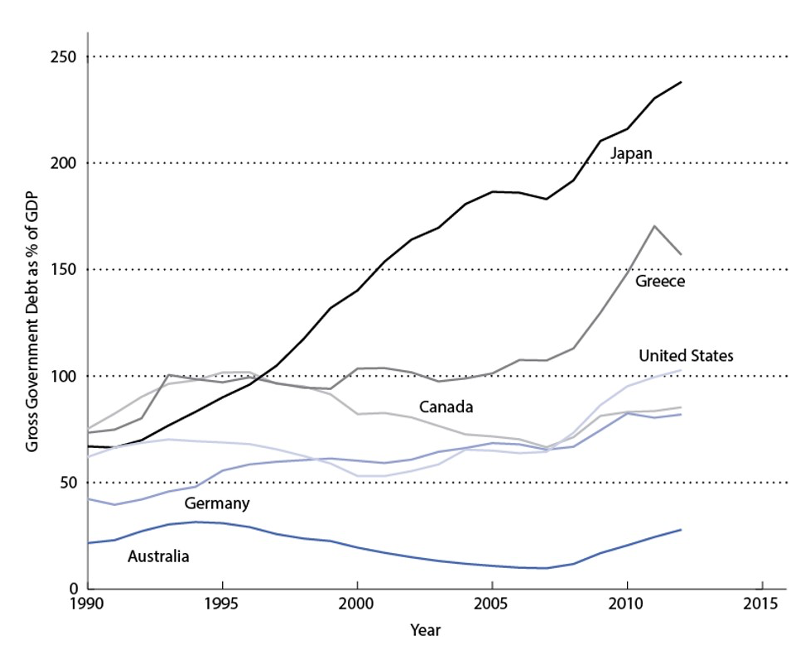
\includegraphics[scale=0.55]{Figures/W_Fig_16pt6.png}
\end{figure}
Greek debt rose by $\approx$ 50\% of GDP!
\end{frame}



\begin{frame}
\frametitle[alignment=center]{Production, Investment, and the Current Account}
\begin{itemize}
\item So far our model of savings=current account is embarassing!
\bigskip
\item There are ways to save other than trade...investment!
\bigskip
\item Getting back to GDP:
$$Y=C+I+G+NX$$
\item World real interest rate is $r^*$, $Y^d$ shifts until it intersects $Y^s$ at $r^*$ \tikz[tstyle]{\node[nstyle](node1){$x$}}
			\begin{tikzpicture}[tpstyle]
				\draw[arrow,->] ([yshift=2pt]node1.north east) to[bend left] +(0.7,+0.3) node[anchor=west] {\hand A comment from the north};
				\draw[arrow,->] ([yshift=-2pt]node1.south) to[bend right] +(1.6,-0.2) node[anchor=west] {\hand A comment from the south};
			\end{tikzpicture}	
\item So if the $r$ that would cause $Y^d=Y^s$ if no trade is too low, you export
\bigskip
\item Let's take a look!
\end{itemize}
\end{frame}

\begin{frame}
\frametitle[alignment=center]{A small open economy model with production and investment}
\begin{figure}
\centering
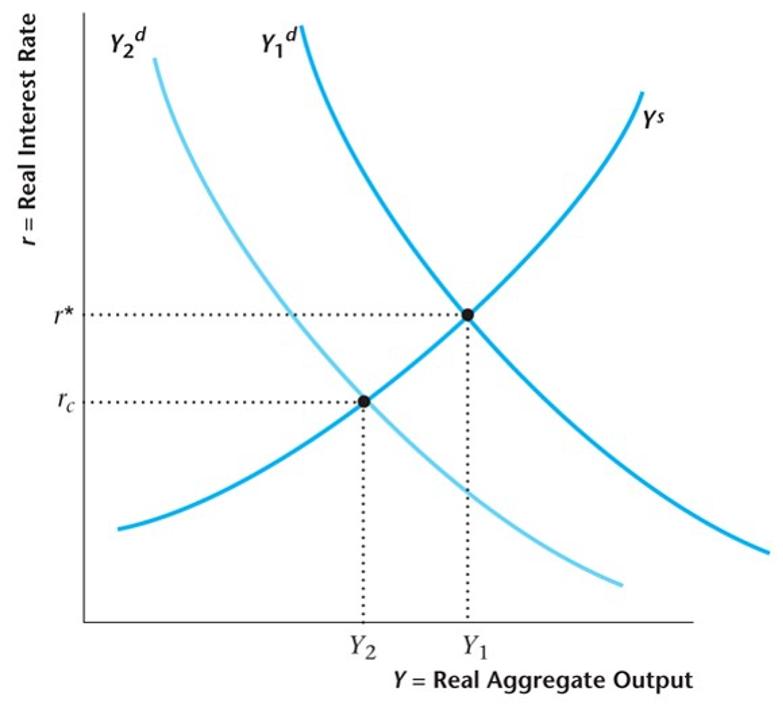
\includegraphics[scale=0.55]{Figures/W_Fig_16pt7.png}
\end{figure}
Possibly easier to think of $r^*$ as determining quantity $Y^d$, and slope is domestic
\end{frame}

\begin{frame}
\frametitle[alignment=center]{Experiment 1: Effects of an Increase in the World Real Interest Rate}
\begin{itemize}
\item Our model is the same as before, except now, rather than $Y^s=Y^d$ determining $r$, world $r$ determines the point at which $Y^d$ intersects $Y^s$ 
\bigskip
\item Take the case in which $r^*$ rises
\bigskip
\item This is a shift out in demand: overall $Y$ increases
\bigskip
\item $I$ decreases (higher MPK required) but $C$ may rise or fall (substitution pushes down, income pushes up)
\end{itemize}
\end{frame}

\begin{frame}
\frametitle[alignment=center]{An increase in the world real interest rate}
\begin{figure}
\centering
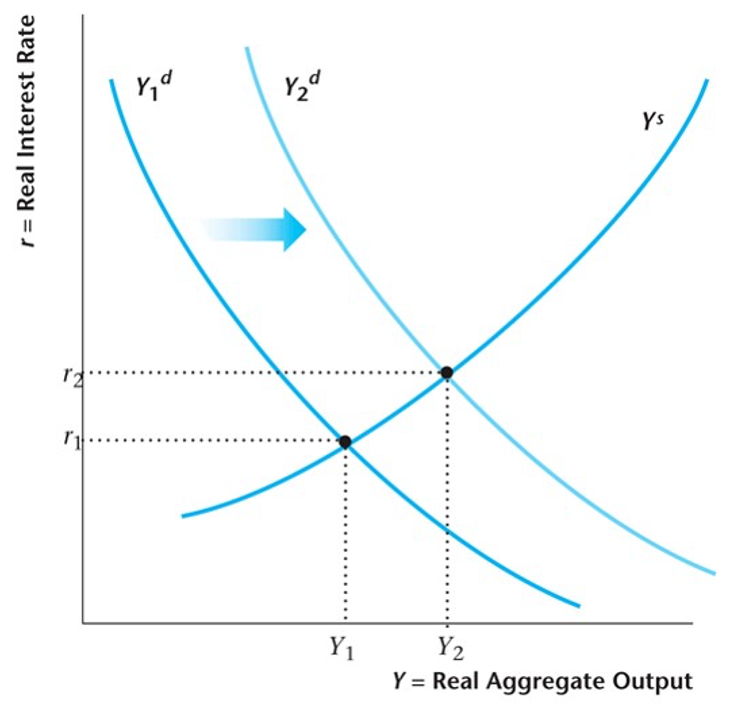
\includegraphics[scale=0.55]{Figures/W_Fig_16pt8.png}
\end{figure}
Possibly easier to think of $r^*$ as determining quantity $Y^d$, and slope is domestic
\end{frame}

\begin{frame}
\frametitle[alignment=center]{Experiment 2: Effects of Government Expenditure on the Current Account}
\begin{itemize}
\item Suppose there's an increase in $G$ (temporary)
\bigskip
\item Negative income effect shifts labor (and thus output supply) out
\bigskip
\item Government demand shifts output demand out, but $r$ stays fixed (world interest rate) so $Y^d$  
\bigskip
\item $Y^d$ increases, but $r$ does not, so no investment or consumption crowding-out  (unlike in Ch. 11!)
\bigskip
\item Here, if $Y$ increases by less than $G$, so overall income increases.  Net exports decline.
\end{itemize}
\end{frame}

\begin{frame}
\frametitle[alignment=center]{A Temporary Increase in Government Spending}
\begin{figure}
\centering
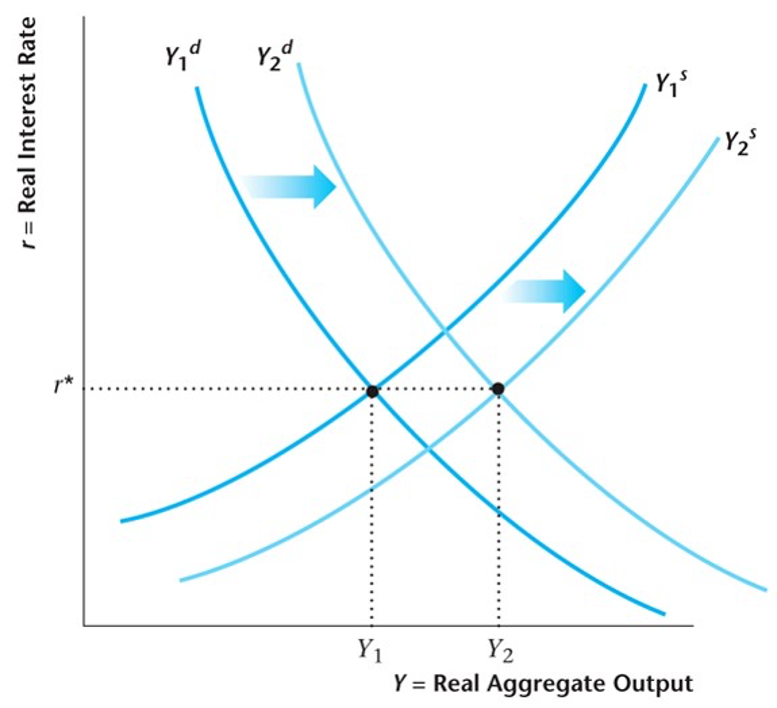
\includegraphics[scale=0.55]{Figures/W_Fig_16pt9.png}
\end{figure}
Possibly easier to think of $r^*$ as determining quantity $Y^d$, and slope is domestic
\end{frame}



\begin{frame}
\frametitle[alignment=center]{Experiment 3: Effects of Increase in TFP Today}
\begin{itemize}
\item Previously, TFP increased labor demand, wages, employment, and output, and decreased the interest rate
\bigskip
\item But now $r$ can't fall (we are small part of global)
\bigskip
\item Now, when $z$ increases, output supply and demand both shift out
\bigskip
\item Output supply increases the current account surplus
\bigskip
\item More income means increased consumption.  Interest rates stay same, so investment constant, $C$ increases
\end{itemize}
\end{frame}

\begin{frame}
\frametitle[alignment=center]{An increase in the current TFP}
\begin{figure}
\centering
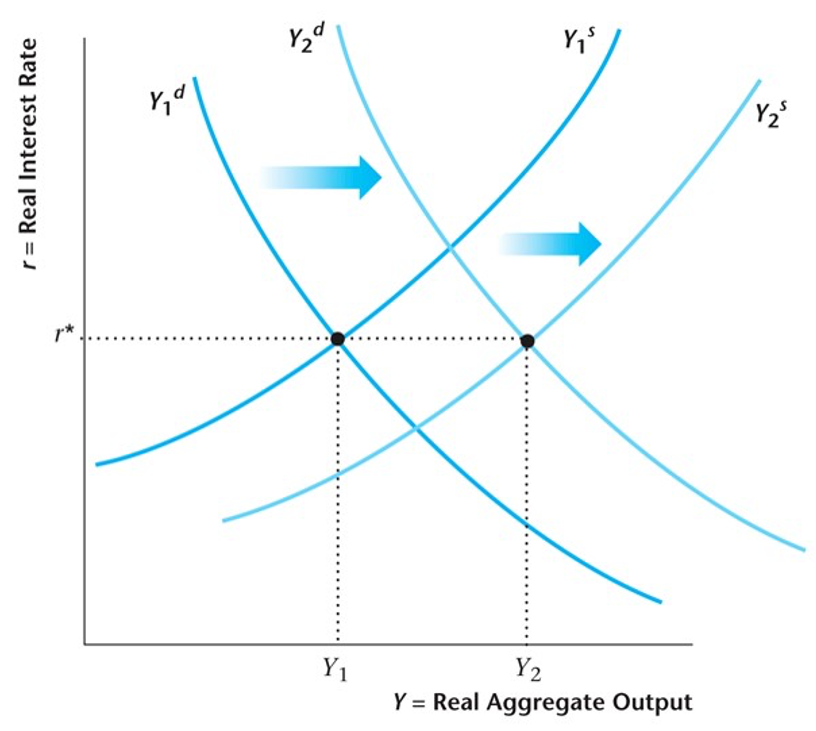
\includegraphics[scale=0.55]{Figures/W_Fig_16pt10.png}
\end{figure}
\end{frame}

\begin{frame}
\frametitle[alignment=center]{Experiment 3: Effects of Increase in TFP in Future}
\begin{itemize}
\item Firm knows increase in future TFP
\bigskip
\item So output demand increases
\bigskip
\item But end output demand fixed, so only crowd-out: current account surplus falls
\bigskip
\item A (true) optimistic boom should reduce current account surplus
\bigskip
\item You see this in the ``dot-com" boom
\end{itemize}
\end{frame}

\begin{frame}
\frametitle[alignment=center]{An increase in the current TFP}
\begin{figure}
\centering
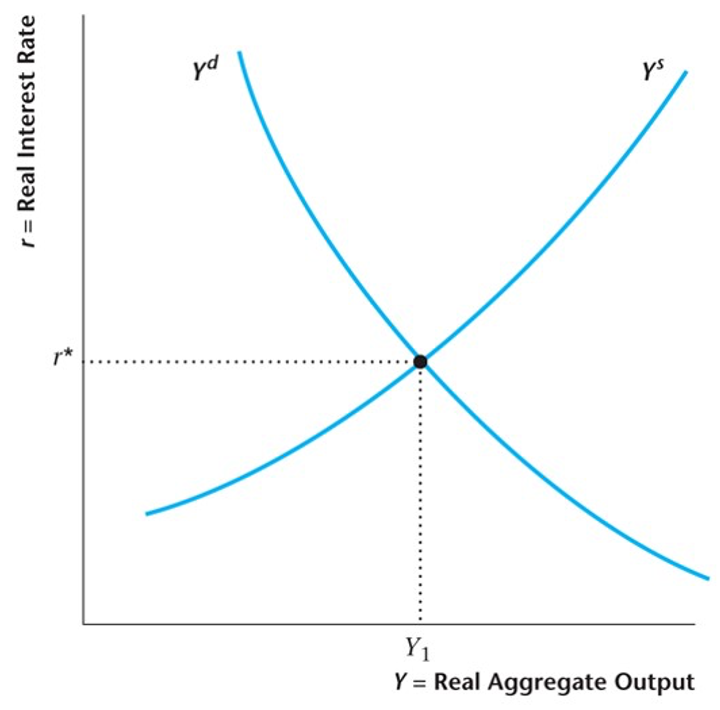
\includegraphics[scale=0.55]{Figures/W_Fig_16pt11.png}
\end{figure}
\end{frame}

\begin{frame}
\frametitle[alignment=center]{Summary}
\begin{itemize}
\item Trade changes our equilibrium a bit
\bigskip
\item Now $r$ is fixed
\bigskip
\item Domestic $Y^d$ is still relevant, it determines current account deficit and surplus
\bigskip
\item Even though total $Y^d$ is set by $r$
\bigskip
\item Some analyses change:  now, govt doesn't crowd out investment, TFP increases don't change interest rates, etc.
\end{itemize}
\end{frame}




\end{document}